\chapter{Implementazione proposta}
\label{chap:implementazione}
\vspace{1cm}
Il Capitolo \ref{chap:approccio} è stato interamente dedicato alla descrizione 
dell'approccio adottato nel lavoro oggetto di questa tesi, al fine di 
realizzare un baseline scheduler che tenga conto di possibili 
\emph{riconfigurazioni} e \emph{comunicazioni}, capace di fornire una 
valutazione quantitativa della bontà di un dato mapping.

Questo capitolo è dedicato alla descrizione dei dettagli implementativi 
riguardanti la realizzazione dell'algoritmo di scheduling.

Il capitolo è strutturato nel seguente modo: la Sezione 
\ref{sec:osservazioniGenerali} fornisce alcune osservazioni preliminari 
riguardo alle scelte implementative del progetto \ac{FASTER}; la Sezione 
\ref{sec:struttureDati} contiene la descrizione delle strutture dati relative 
all'implementazione dello scheduler; la Sezione \ref{sec:classiGerarchie} 
descrive le classi e le gerarchie che compongono la parte della toolchain 
relativa alla parte di mapping/scheduling (Sezione 
\ref{subsec:algoritmoEsplorazione}) e i componenti dell'algoritmo di scheduling 
nel dettaglio (Sezione \ref{subsec:algoritmoScheduling}).


\section{Osservazioni generali}
\label{sec:osservazioniGenerali}
La maggior parte della toolchain di \ac{FASTER} è sviluppata in C++, 
linguaggio di programmazione a oggetti sviluppato da Bjarne Stroustrup 
\cite{CppStroustrup} come miglioramento del C, creato invece da Dennis Ritchie 
\cite{CKernighanRitchie}. La parte di interfaccia grafica, chiamata \emph{ASAP 
GUI} è sviluppata in C\#, linguaggio di programmazione ad oggetti sviluppato da 
Microsoft nell'ambito del \emph{framework .NET} \cite{ProCSharp}. ASAP GUI 
lancia degli script scritti in Python \cite{ThinkPython}, che si occupano di 
modificare l'XML del file di progetto come specificato dall'utente tramite 
l'interfaccia grafica.
% FIXME scrivere dei backend in python?
\paragraph{Convenzioni implementative della toolchain}
Riguardo allo sviluppo in C++ della toolchain di \ac{FASTER}, si è deciso di 
usare le strutture (\verb+struct+), per indicare tipi di dati dedicati alla 
memorizzazione di informazioni o utilizzati come ``contenitori''; le classi 
(\verb+class+) vengono utilizzate invece per rappresentare oggetti che hanno 
degli algoritmi al loro interno, invocabili come metodi.

\paragraph{Organizzazione dei namespace}
Nel codice si è deciso di includere le strutture e le classi dentro a 
\emph{namespace}, allo scopo di prevenire eventuali conflitti di nomi e di 
organizzare logicamente per categorie le varie parti della toolchain.

\begin{figure}
 \begin{center}
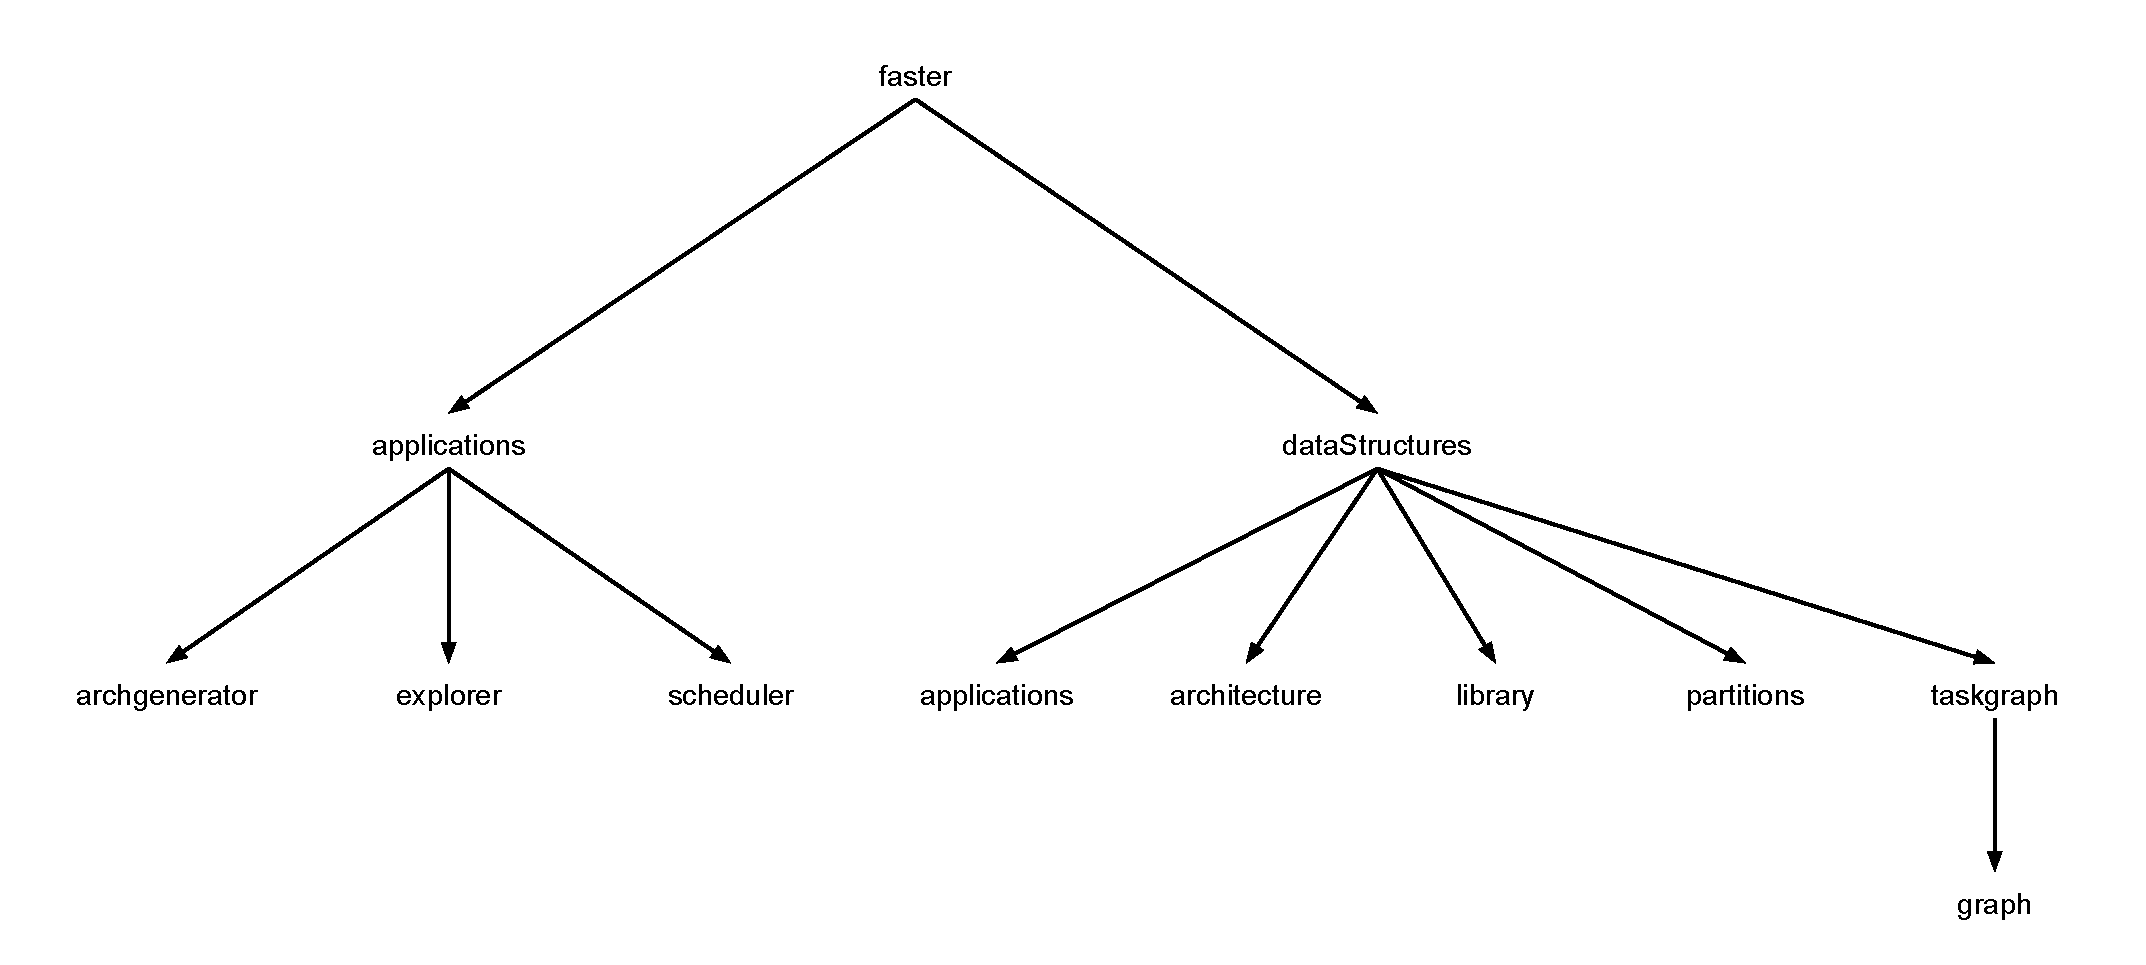
\includegraphics[width=\textwidth]{capitoli/figure/cap4/FASTERNamespaces.pdf}
\caption{Gerarchia dei namespace di \acs{FASTER}.}
\label{fig:gerarchiaNamespace}
 \end{center}
\end{figure}

Una rappresentazione della struttura dei namespace è visibile in Figura 
\ref{fig:gerarchiaNamespace}. La maggior parte di questi namespace verrà 
spiegata al momento di trattare classi o strutture che ne fanno parte 
e sono rilevanti per il lavoro oggetto della tesi.

\paragraph{Convenzioni nell'assegnazione dei nomi}
È stata scelta la seguente convenzione per nominare i dati membro o i metodi 
delle strutture/classi:
\begin{itemize}
 \item nomi di dati membro o metodi aventi specificatore di accesso 
\verb+public+ o \verb+protected+ sono scritti normalmente;
 \item nomi di dati membro o metodi aventi specificatore di accesso 
\verb+private+ sono scritti aggiungendo la stringa ``\verb+m_+'' come prefisso.
\end{itemize}

Eventuali tipi di dato ridefiniti tramite l'uso di \verb+typedef+ iniziano 
con una lettera maiuscola e sono scritti aggiungendo la stringa ``\verb+_t+'' 
come suffisso.

\paragraph{Puntatori e librerie esterne}
Allo scopo di prevenire il verificarsi di \emph{memory leak} difficili da 
identificare e debuggare, si è deciso all'inizio della progettazione di non 
utilizzare i puntatori standard forniti dal linguaggio C++, in favore degli 
shared pointer delle librerie \emph{Boost} \cite{BoostLibrary, BoostSharedPtr}.
Infatti, un oggetto di tipo \verb+boost::shared_ptr+ gestisce automaticamente 
la distruzione dell'oggetto a cui si riferisce una volta che l'ultimo shared 
pointer che punta all'oggetto è distrutto.

L'utilizzo degli shared pointer permette di istanziare l'oggetto tramite 
allocazione dinamica una sola volta, utilizzando poi i puntatori associati per 
l'accesso ai suoi dati e metodi o per il passaggio come parametro.

Nel codice sorgente della toolchain sono presenti delle \verb+typedef+ globali 
aventi il suffisso ``\verb+Ptr+'' che semplificano la definizione degli shared 
pointer per alcune strutture/classi del progetto; ad esempio, alla classe 
\verb+FasterTask+, che identifica un task (generico), corrisponde lo shared 
pointer \verb+FasterTaskPtr+.

% TODO parlare di compilazione, CMake e librerie

\section{Strutture dati}
\label{sec:struttureDati}
In questa sezione vengono presentate alcune strutture dati della toolchain. La 
sezione si divide in due sotto-sezioni: la Sezione 
\ref{subsec:struttureDatiFaster} presenta le strutture dati generali della 
toolchain, non relative allo scheduler; la Sezione 
\ref{subsec:struttureDatiScheduler} presenta invece le strutture utilizzate 
dall'algoritmo di scheduling.


\subsection{\acs{FASTER}}
\label{subsec:struttureDatiFaster}
% TODO


\subsection{Scheduler}
\label{subsec:struttureDatiScheduler}
L'obiettivo di questa sezione è presentare le più importanti strutture dati 
utilizzate dallo scheduler, che si trovano nella cartella 
\emph{toolchain/sources/common/datastructures/cpp/fasterInterfaces/scheduler}. 
Tutte le strutture che saranno esaminate in questa sezione appartengono al 
namespace \verb+faster::applications::scheduler+.

\subsubsection{Scheduler input}
I file \emph{schedulerInput.hpp} e \emph{schedulerInput.cpp} contengono la 
dichiarazione e l'implementazione della struttura \verb+SchedulerInput+, 
rispettivamente.

Il seguente frammento di codice mostra le parti rilevanti della 
dichiarazione della struttura.
\newline
\begin{minted}[frame=single,fontsize=\small,gobble=2,mathescape]{c}
  struct SchedulerInput {
  private:
      FasterProjectPtr m_fasterProject;
      explorer::ExplorerTrace m_explorerTrace;
      std::vector<FasterTaskPtr> m_topologicalSorting;
      CriticalPathInfoMap_t m_criticalPathInfo;
      std::vector<ProcessingTaskPair_t> m_reconfigurationsList;
      bool m_busAvailable;
      FasterTaskGraphPtr m_taskGraph;
      FasterReconfigurationElementPtr m_reconfigurationController;
      FasterMemoryElementPtr m_ramElement;
      FasterCommunicationElementPtr m_busElement;
      SchedulerMemoryManagerPtr m_memoryManager;
      int m_readPortsNum;
      int m_writePortsNum;
      // code...
  };
\end{minted}
La struttura \verb+SchedulerInput+ contiene i dati principali che vengono usati 
dallo scheduler nel corso dell'elaborazione, dal preprocessing allo scheduling 
effettivo. In particolare, si notano il puntatore alla struttura 
\verb+FasterProject+, che è necessaria per accedere alle informazioni 
sull'architettura e sull'applicazione, come spiegato nella sezione precedente.
Il dato membro \verb+m_taskGraph+ viene impostato in seguito alla fase di 
preprocessing, e contiene in task graph arricchito delle comunicazioni e 
riconfigurazioni da considerare nella fase di scheduling vera e propria. 
\verb+m_explorerTrace+ contiene la lista di triple calcolata dal mapper per 
l'iterazione corrente dell'esplorazione.

Oltre a questi, vi sono anche dei puntatori al gestore della memoria e ai 
componenti di riconfigurazione e di comunicazione (\acs{RAM} e BUS, se 
presente), il numero di porte di lettura/scrittura disponibili sulla \acs{RAM} 
e variabili aggiuntive che contengono le informazioni di percorso critico dei 
task, dei task ordinati topologicamente e della lista delle riconfigurazioni.

\subsubsection{Scheduler Data}
I file \emph{schedulerData.hpp} e \emph{schedulerData.cpp} contengono il codice 
sorgente della struttura \verb+SchedulerData+, che contiene dati continuamente 
aggiornati durante l'esecuzione dell'algoritmo di scheduling. A differenza dei 
dati contenuti in \verb+SchedulerInput+, questi dati sono racchiusi in una 
struttura a sé stante perchè figurino come logicamente separati dai dati che 
invece fanno parte dell'input dell'algoritmo.

Viene ora presentato un frammento di codice rilevante per la dichiarazione 
della struttura.
\newline
\begin{minted}[frame=single,fontsize=\small,gobble=2,mathescape]{c}
  struct SchedulerData {
      TaskSet_t unscheduledTasksSet;
      std::vector<FasterTaskPtr> scheduledTasksList;
      std::vector<FasterTaskPtr> readyTasksList;
  };
\end{minted}
Come si può vedere, la struttura contiene l'insieme dei task non ancora 
selezionati per lo scheduling e i vettori dei task già schedulati e pronti per 
essere schedulati. Si è deciso di incapsulare questi dati in una struttura 
modificabile da tutti i componenti dell'algoritmo perchè alcuni componenti 
potrebbero dover fare delle modifiche on-the-fly\footnote{Ad esempio, nel caso 
la policy di scheduling delle comunicazioni scelga di utilizzare il BUS come 
mezzo di comunicazione, il task \emph{READ} corrispondente dev'essere 
eliminato dalla lista dei task rimanenti.}.

\subsubsection{Scheduler Gantt}
La struttura \verb+SchedulerGantt+ è definita nei file 
\emph{schedulerGantt.hpp} e \emph{schedulerGantt.cpp}; la struttura contiene il 
diagramma di Gantt utilizzato dall'algoritmo per visualizzare la soluzione 
calcolata. All'inizio dell'elaborazione il diagramma è vuoto, viene 
progressivamente riempito con le informazioni di scheduling calcolate ad ogni 
passo.

Vengono inizialmente ridefiniti alcuni tipi di dato, per semplificare la 
scrittura e la lettura del codice.
\newline
\begin{minted}[frame=single,fontsize=\small,gobble=2,mathescape]{c}
  typedef std::set<ScheduledTaskInfo> BusyInfoSeries_t;
  typedef std::unordered_map<std::string, BusyInfoSeries_t> GanttMap_t;
\end{minted}

Nel seguente frammento di codice sono illustrate le parti rilevanti della 
dichiarazione della struttura.
\newline
% FIXME aggiustare indentazione codice
\begin{minted}[frame=single,fontsize=\small,gobble=2,mathescape]{c}
  struct SchedulerGantt {
      private:
          GanttMap_t m_gantt;
          // code...
      public:
          // code...
          void addBusyInfo(const ScheduledTaskInfo & timeInfo);
          bool isOverlapping(const FasterComponentPtr & elem,
                             const ScheduledTaskInfo & timeInfo) const;
          bool isComponentBusy(const FasterComponentPtr & elem,
                               long int timestamp) const;
          std::unordered_map<std::string, BusyInfoSeries_t> 
              getBusyComponentsGivenTime(long int timestamp) const;
          BusyInfoSeries_t getBusyInfoGivenComponentAndTime(
            const FasterComponentPtr & elem,
            long int timestamp) const;
          long int getFirstAvailableTime(
            const FasterComponentPtr & elem, 
            long int timestamp, long int execTime) const;
          // code...
  };
\end{minted}
Il diagramma di Gantt è quindi rappresentato tramite una mappa non ordinata 
che ha per chiavi delle stringhe, gli id dei componenti, e per valori un 
insieme di \verb+ScheduledTaskInfo+, struttura che contiene le informazioni di 
scheduling di un task.

Sono a disposizione dei metodi pubblici per aggiungere le informazioni di 
scheduling relative a un task, per verificare se un determinato componente è 
occupato in un determinato istante di tempo e per ottenere il primo istante di 
tempo in cui un determinato componente è libero.

\subsubsection{Scheduler Output}
I file \emph{schedulerOutput.hpp} e \emph{schedulerOutput.cpp} contengono la 
dichiarazione e la definizione della struttura \verb+SchedulerOutput+. Questa 
struttura contiene i dati di output dello scheduler, che vengono 
progressivamente aggiornati man mano che l'esecuzione dell'algoritmo avanza, e 
alla fine sono utilizzati per il calcolo della metrica \emph{makespan}.


Nel seguente frammento di codice sono presentate le ridefinizioni di tipo di 
dato utilizzate in \emph{schedulerOutput.hpp}.
\newline
\begin{minted}[frame=single,fontsize=\small,gobble=2,mathescape]{c}
  typedef std::tr1::tuple<FasterTaskPtr,
                          FasterComponentPtr, 
                          FasterImplementationPtr> MappingStep_t;
  typedef std::unordered_map<FasterTaskPtr,
                             ScheduledTaskInfo, 
                             utilities::HashUtility<FasterTaskPtr>, 
                             utilities::EqualUtility<FasterTaskPtr> > 
                             ScheduledTaskInfoMap_t;
\end{minted}

La seguente porzione di codice illustra invece la dichiarazione della struttura 
\verb+SchedulerOutput+.
\newline
\begin{minted}[frame=single,fontsize=\small,gobble=2,mathescape]{c}
  struct SchedulerOutput {
      private:
          SchedulerGantt m_schedulingGantt;
          ScheduledTaskInfoMap_t m_scheduledTaskInfo;
          std::set<MappingStep_t> m_schedulerMapping;

      public:
          // code...
          void addSchedulingTimeInfo(const ScheduledTaskInfo & timeInfo);
          void addScheduledTaskInfo(const FasterTaskPtr & task,
                  const ScheduledTaskInfo & info);
          long int computeMakespan() const;
  };
\end{minted}
Come si può vedere dal codice, la struttura agisce come wrapper attorno ai 
metodi della struttura \verb+SchedulerGantt+ vista in precedenza, ed espone dei 
metodi che permettono di aggiungere all'output le informazioni di scheduling 
appena calcolate. Il metodo \verb+computeMakespan()+ permette di calcolare la 
metrica di valutazione dello scheduling. Nella struttura sono presenti dati 
membro aggiuntivi che rendono meglio accessibili le informazioni di scheduling 
già ricavabili dal diagramma di Gantt. Da queste variabili aggiuntive è 
possibile ricavare in maniera banale le informazioni per ogni task tramite la 
mappa \verb+m_scheduledTaskInfo+ e il mapping assegnato dallo scheduler tramite 
la variabile \verb+m_schedulerMapping+\footnote{Mentre il mapping determinato 
dal mapper è specificato solamente per processing task (relativi al task 
graph originale), il mapping presente nell'output dello scheduler è relativo ai 
task del task graph preprocessato.}.

\subsubsection{Scheduler Utility}
I file \emph{schedulerUtility.hpp} e \emph{schedulerUtility.cpp}, infine, 
contengono la definizione di alcune strutture comunemente utilizzate dallo 
scheduler e viste anche nei precedenti frammenti di codice sorgente.

La struttura \verb+TaskTimes+ incapsula gli istanti di inizio e fine di un task.
\newline
\begin{minted}[frame=single,fontsize=\small,gobble=2,mathescape]{c}
  struct TaskTimes {
      long int startTime;
      long int endTime;
      // constructor, destructor and operators
  };
\end{minted}

La struttura \verb+CriticalPathInfo+ contiene le informazioni relative al 
percorso critico di un task.
\newline
\begin{minted}[frame=single,fontsize=\small,gobble=2,mathescape]{c}
  struct CriticalPathInfo {
      long int asap;
      long int alap;
      long int slack;
  };
\end{minted}

La struttura \verb+ScheduledTaskInfo+ contiene le informazioni riguardanti lo 
scheduling di un task.
\newline
\begin{minted}[frame=single,fontsize=\small,gobble=2,mathescape]{c}
  struct ScheduledTaskInfo {
      FasterTaskPtr task;
      FasterImplementationPtr implementation;
      FasterComponentPtr component;
      TaskTimes times_info;
      long int executionTime;
      // operators
  };
\end{minted}

La struttura \verb+MemoryOccupationInfo+ contiene le informazioni relative a 
un'area di memoria che viene allocata a un processing task.
\newline
\begin{minted}[frame=single,fontsize=\small,gobble=2,mathescape]{c}
  struct MemoryOccupationInfo {
      unsigned long base_addr;
      unsigned long data_size;
      TaskSet_t consumersSet;
      bool reusable_area;
  };
\end{minted}

Infine, all'interno del file \emph{schedulerUtility.cpp} è presente un 
namespace \verb+utilities+, che contiene due strutture che hanno l'operatore 
\verb+()+ ridefinito. Queste strutture vengono utilizzate per testare 
l'equivalenza o per calcolare l'hash di un oggetto del tipo specificato tramite 
template. Vengono utilizzate nelle mappe e negli insiemi non ordinati mostrati 
nelle strutture precedenti, e operano sul dato membro ``\verb+id+'' 
dell'oggetto passato come parametro.


\section{Classi e gerarchie principali}
\label{sec:classiGerarchie}
In questa sezione vengono presentate le classi principali della toolchain 
relativa all'algoritmo di esplorazione (mapper) e in particolare 
dell'algoritmo di scheduling utilizzato per la valutazione quantitativa della 
soluzione proposta dal mapper.

\subsection{Algoritmo di esplorazione}
\label{subsec:algoritmoEsplorazione}
Il codice sorgente dell'algoritmo di esplorazione è localizzato nella cartella 
\emph{toolchain/sources/explorer}. L'eseguibile dell'algoritmo di esplorazione 
è compilato a partire dal \verb+main()+ che si trova nel file sorgente 
\emph{explorerMain.cpp} nella suddetta cartella. Il main si occupa di 
istanziare i vari componenti che verranno spiegati nelle prossime sezioni e di 
lanciare la procedura di esplorazione. Al termine, viene generato un file di 
output e stampate le statistiche dell'esplorazione.

\subsubsection{Componente di esplorazione}
Il componente di esplorazione viene istanziato dalla funzione \verb+main()+ e 
si occupa di gestire l'esplorazione dal momento del lancio effettuato nel main, 
fino alla terminazione. Il codice di questo componente è contenuto nei file 
\emph{explore.hpp} ed \emph{explore.cpp}, presenti nella sottocartella 
\emph{explore}.

Poichè il componente di esplorazione rappresenta un oggetto contenente un 
algoritmo invocabile, secondo la convenzione implementativa indicata nella 
Sezione \ref{sec:osservazioniGenerali}, è implementato come \verb+class+ e 
inserito nel namespace \verb+faster::applications::explorer+, come tutti i 
componenti che vedremo di seguito relativi all'algoritmo di esplorazione.

Il componente di esplorazione ha una propria interfaccia di input, definita 
nella struttura \verb+ExplorerInput+, contenuta nella cartella 
\emph{toolchain/sources/common/datastructures/cpp/fasterInterfaces/explorer}. 
Al suo interno presenta dei riferimenti ai componenti di iterazione e di 
terminazione. Entrambi questi componenti verranno descritti nelle prossime 
sezioni, e si trovano nella sottocartella \emph{explore/exploreComponents}.

\subsubsection{Componente di iterazione}
Data l'ampia modularità decisa in fase di progettazione, il componente di 
iterazione è rappresentato da una classe astratta che espone 
\verb+nextIteration()+, un metodo virtuale puro\footnote{Un metodo virtuale 
puro deve essere implementato da tutte le sottoclassi della classe che lo 
dichiara.} che si occupa di gestire una iterazione dell'esplorazione.

L'interfaccia della classe astratta è definita in 
\emph{explore/exploreComponents/iteration/exploreIterationAlgorithm.hpp}; è 
presente anche una sottoclasse che implementa la funzionalità iterativa, nella 
sottocartella \emph{explore/exploreComponents/iteration/aco}. In ogni caso si 
può estendere aggiungendo altri componenti come sottoclassi separate che 
ridefiniscono il metodo per l'iterazione.
\newline
\begin{minted}[frame=single,fontsize=\small,gobble=2,mathescape]{c}
  class ExploreIterationAlgorithm {
      protected:
          const ExplorerInput& m_explorerInput;
      public:
          // constructor and destructor
          virtual std::set<ExplorerOutput> nextIteration() = 0;
          virtual ExplorerOutput getCurrentBestSolution() const = 0;
          virtual std::set<ExplorerOutput> getLastIterationSolutions()
              const = 0;
  };
\end{minted}


\subsubsection{Componente di terminazione}
La terminazione dell'algoritmo di esplorazione viene decisa dal componente di 
terminazione. Come per l'iterazione, anche il componente di iterazione è 
composto da una classe astratta che espone un metodo che deve essere 
reimplementato dalle sottoclassi, \verb+isTerminated()+.

Come nel caso del componente di iterazione, è presente un'implementazione della 
classe astratta, che termina quando il numero di iterazioni raggiunge il limite 
specificato nel file di configurazione dell'explorer.
\newline
\begin{minted}[frame=single,fontsize=\small,gobble=2,mathescape]{c}
  class ExploreTerminationAlgorithm {
      protected:
          const ExplorerInput & m_sd;
      public:
          // constructor and destructor
          virtual bool isTerminated() const = 0;
          virtual void updateState(std::set<ExplorerOutput>) = 0;
          virtual faster::dataStructures::FasterPerformanceStatistics 
              getStatistics() = 0;
  };
\end{minted}

% TODO metriche dell'algoritmo di esplorazione

\subsection{Algoritmo di scheduling}
\label{subsec:algoritmoScheduling}
L'obiettivo di questa sezione è presentare le porzioni più importanti del 
codice dell'algoritmo di scheduling. Le interfacce di input/output e le 
strutture dati utilizzate sono già state descritte nella Sezione 
\ref{subsec:struttureDatiScheduler}, in questa sezione verranno esaminati i 
vari componenti dello scheduler che gestiscono l'elaborazione.

Il codice sorgente dell'algoritmo di scheduling è contenuto nella cartella 
\emph{toolchain/sources/scheduler}; la sua struttura rispecchia quella 
dell'algoritmo di esplorazione, come verrà spiegato nelle prossime sezioni per 
l'esame dei componenti dello scheduler. Tutte le classi che compongono 
sono incluse nel namespace \verb+faster::applications::scheduler+.


